
%(BEGIN_QUESTION)
% Copyright 2006, Tony R. Kuphaldt, released under the Creative Commons Attribution License (v 1.0)
% This means you may do almost anything with this work of mine, so long as you give me proper credit

Ledningsevne i vannbaserte løsninger uttrykkes vanligvis i Siemens per centimeter (S/cm). Siemens er den inverse av Ohm, siden ledningsevne ($G$) og motstand ($R$) er inverse størrelser:

$$G = {1 \over R}$$

Vi kan måle ledningsevne i en væske ved å senke to elektroder med kjent areal ned i væsken, holde kjent avstand mellom dem, og måle ledningsevnen mellom elektrodene. Enheten kalles en {\it ledningsevnecelle}:

$$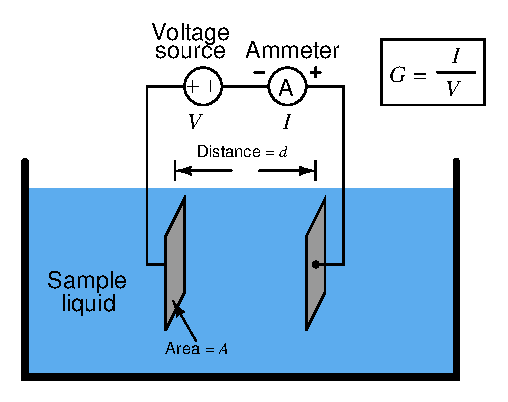
\includegraphics[width=15.5cm]{i00606x01.eps}$$

Hvis væskens ledningsevne ikke endres, hvordan påvirkes målingen av endringer i elektrodeareal og avstand? Følgende ligning kan være nyttig:

$$G = k{A \over d}$$

\noindent
Der,

$G$ = Ledningsevne i Siemens (S)

$k$ = Spesifikk ledningsevne i Siemens per centimeter (S/cm)

$A$ = Elektrodeareal (hver), i cm$^{2}$

$d$ = Elektrodeavstand, i cm

\vskip 10pt

Vis også hvordan enheten ``Siemens per centimeter'' følger direkte fra denne ligningen.

\underbar{file i00606}
%(END_QUESTION)





%(BEGIN_ANSWER)

Her er en versjon av ligningen med enheter i stedet for variabler:

$$[\hbox{S}] = \left[{\hbox{S} \over \hbox{cm}}\right]{[\hbox{cm}^2] \over [\hbox{cm}]}$$

\vskip 10pt

Oppfølgingsspørsmål: oppgi en eldre enhet for ledningsevne brukt før Siemens. Hint: den er faktisk {\it meningsfull} i navnet.

%(END_ANSWER)





%(BEGIN_NOTES)

Ledningsevnen avtar med økende areal ($A$), og øker med økende avstand ($d$).

\vskip 10pt

Den gamle enheten for ledningsevne er {\it mho}: ``ohm'' skrevet baklengs. Symbolet var til og med en opp-ned gresk stor omega.

%INDEX% Måling, analytisk: ledningsevne

%(END_NOTES)

